\noindent

\includegraphics[height=1.25cm]{images/pictograms/replication}

\includegraphics[height=1.25cm]{images/pictograms/benchmark}

\includegraphics[height=1.25cm]{images/pictograms/under_construction}

\includegraphics[height=1.25cm]{images/pictograms/tools}

\includegraphics[height=1.25cm]{images/pictograms/FEM}

\includegraphics[height=1.25cm]{images/pictograms/paraview}

%%%%%%%%%%%%%%%%%%%%%%%%%%%%%%%%%%%%%%%%%%%%%%%%%%%%%%%%%%%%%%%%%%%%%%%%%%%%%%%%%%%%%%%%%%%%%%%%%%%

\begin{flushright} {\tiny {\color{gray} python\_codes/fieldstone\_174/text.tex}} \end{flushright}

%\lstinputlisting[language=bash,basicstyle=\small]{python_codes/template_keywords.key}

\par\noindent\rule{\textwidth}{0.4pt}

\begin{center}
\inpython
{\small Code: \url{https://github.com/cedrict/fieldstone/tree/master/python_codes/fieldstone_174}}
\end{center}

\par\noindent\rule{\textwidth}{0.4pt}

Last revision: June 16th, 2025.

\par\noindent\rule{\textwidth}{0.4pt}

%%%%%%%%%%%%%%%%%%%%%%%%%%%%%%%%%%%%%%%%%%%%%%%%%%%%%%%%%%%%%%%%%%%%%%%%%%%%%%%%%%%%%%%%%%%%%%%%%%%

The motivation for this \stone originates in \textcite{zibz98} (1998):

\begin{center}
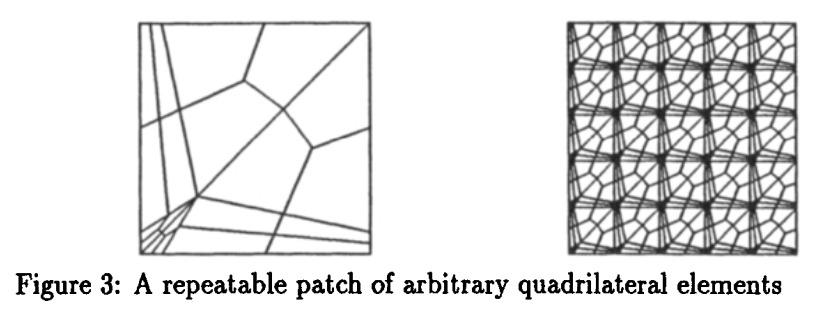
\includegraphics[width=8cm]{python_codes/fieldstone_174/images/zibz98a}\\
{\captionfont See also Fig.~4 of the paper.}
\end{center}

In essence, we wish to write a function that generates a mesh like the 
one in the figure above.  

Note that what follows actually replicates Fig.~4e of the paper, which is
similar to the figure above but not identical (check lower left corner).
In order to build the mesh we need to label the nodes of the 'master' cell 
which is decomposed in 18 sub-elements:

\begin{center}
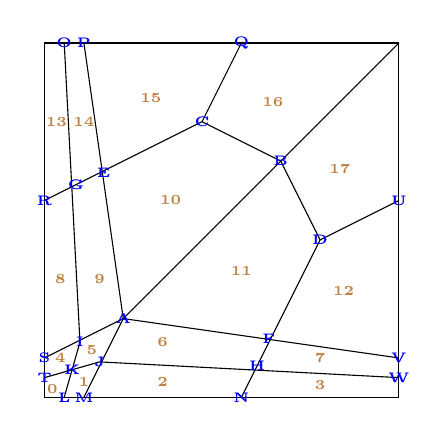
\begin{tikzpicture}
\draw[thin] (0,0) -- (4.5,0) -- (4.5,4.5) -- (0,4.5) -- cycle;  
\draw[thin] (1,1) -- (4.5,4.5) ; %AB
\draw[thin] (0,2.5) -- (2,3.5) -- (3,3) -- (3.5,2) -- (2.5,0); % RCBDN
\draw[thin] (3.5,2) -- (4.5,2.5); %DR
\draw[thin] (2,3.5) -- (2.5,4.5) ; %CN
\draw[thin] (0.5,0) -- (1,1) -- (0.5,4.5) ; % MAM
\draw[thin] (0,0.5) -- (1,1) -- (4.5,0.5) ; % SAS
\draw[thin] (0.25,0) -- (0.45,0.7) -- (0.25,4.5) ; % LIL
\draw[thin] (0,0.25) -- (0.7,0.45) -- (4.5,0.25) ; % TJT

\node[blue] at (1,1) {\tiny \bf A};
\node[blue] at (3,3) {\tiny \bf B};
\node[blue] at (2,3.5) {\tiny \bf C};
\node[blue] at (3.5,2) {\tiny \bf D};
\node[blue] at (0.75,2.85) {\tiny \bf E};
\node[blue] at (2.85,0.75) {\tiny \bf F};
\node[blue] at (0.4,2.7) {\tiny \bf G};
\node[blue] at (2.7,0.4) {\tiny \bf H};
\node[blue] at (0.45,0.7) {\tiny \bf I};
\node[blue] at (0.7,0.45) {\tiny \bf J};
\node[blue] at (0.35,0.35) {\tiny \bf K};
\node[blue] at (0.25,0) {\tiny \bf L};
\node[blue] at (0.5,0) {\tiny \bf M};
\node[blue] at (2.5,0) {\tiny \bf N};
\node[blue] at (0.25,4.5) {\tiny \bf O};
\node[blue] at (0.5,4.5) {\tiny \bf P};
\node[blue] at (2.5,4.5) {\tiny \bf Q};
\node[blue] at (0,0.25) {\tiny \bf T};
\node[blue] at (0,0.5) {\tiny \bf S};
\node[blue] at (0,2.5) {\tiny \bf R};
\node[blue] at (4.5,0.25) {\tiny \bf W};
\node[blue] at (4.5,0.5) {\tiny \bf V};
\node[blue] at (4.5,2.5) {\tiny \bf U};

\node[brown] at (0.1,0.1) {\tiny \bf 0};
\node[brown] at (0.5,0.2) {\tiny \bf 1};
\node[brown] at (1.5,0.2) {\tiny \bf 2};
\node[brown] at (3.5,0.15) {\tiny \bf 3};
\node[brown] at (0.2,0.5) {\tiny \bf 4};
\node[brown] at (0.6,0.6) {\tiny \bf 5};
\node[brown] at (1.5,0.7) {\tiny \bf 6};
\node[brown] at (3.5,0.5) {\tiny \bf 7};
\node[brown] at (0.2,1.5) {\tiny \bf 8};
\node[brown] at (0.7,1.5) {\tiny \bf 9};
\node[brown] at (1.6,2.5) {\tiny \bf 10};
\node[brown] at (2.5,1.6) {\tiny \bf 11};
\node[brown] at (3.8,1.35) {\tiny \bf 12};
\node[brown] at (0.15,3.5) {\tiny \bf 13};
\node[brown] at (0.5,3.5) {\tiny \bf 14};
\node[brown] at (1.35,3.8) {\tiny \bf 15};
\node[brown] at (2.9,3.75) {\tiny \bf 16};
\node[brown] at (3.75,2.9) {\tiny \bf 17};
\end{tikzpicture}
\end{center}

We can now look at a mesh composed of $3\times 2$ of these cells.
We have then
\begin{eqnarray}
N_1&=&(nelx+1)*(nely+1) = 4*3 = 12 \text{ (corners of Q1 mesh)} \nn\\
N_2&=&nel*11  = 6*11=66         \text{ (inside nodes)}\nn\\
N_3&=&3*(nelx+1)*nely =3*4*2=24 \text{ (vertical sides nodes)}\nn\\
N_4&=&3*(nely+1)*nelx =3*3*3 = 27 \text{ (horizontal sides nodes)} \nn\\
N&=&N_1+N_2+N_3+N_4=129 \nn
\end{eqnarray}

The resulting mesh is then as follows:

\begin{center}
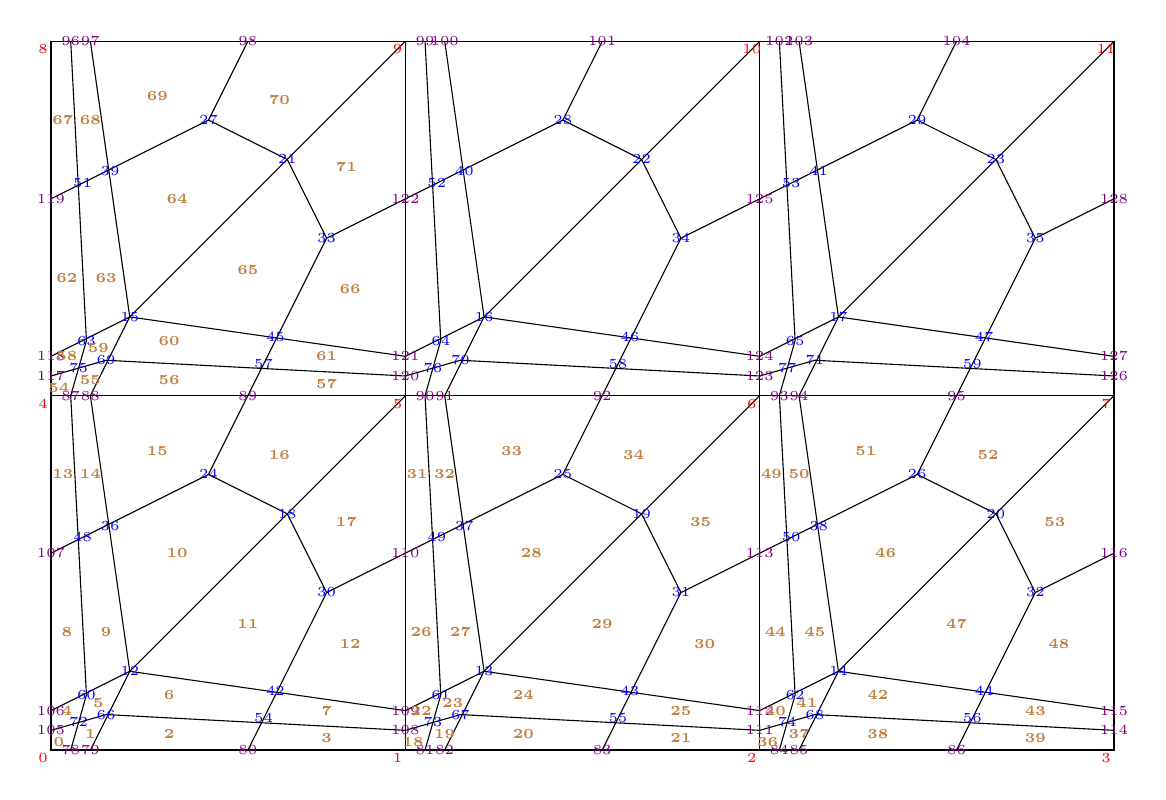
\begin{tikzpicture}
%\draw[step=0.5cm,gray,very thin] (0,0) grid (15,10); %background grid

\draw[thin] (0,0) -- (13.5,0) -- (13.5,9) -- (0,9) -- cycle;  
\draw[thin] (0,4.5) -- (13.5,4.5) ;
\draw[thin] (4.5,0) -- (4.5,9) ;
\draw[thin] (9,0) -- (9,9) ;

%AB line
\draw[thin] (1,1) -- (4.5,4.5) ;
\draw[thin] (1+4.5,1) -- (4.5+4.5,4.5) ;
\draw[thin] (1+9,1) -- (4.5+9,4.5) ;
\draw[thin] (1,1+4.5) -- (4.5,4.5+4.5) ;
\draw[thin] (1+4.5,1+4.5) -- (4.5+4.5,4.5+4.5) ;
\draw[thin] (1+9,1+4.5) -- (4.5+9,4.5+4.5) ;

%RCBDN
\draw[thin] (0,2.5) -- (2,3.5) -- (3,3) -- (3.5,2) -- (2.5,0);
\draw[thin] (0+4.5,2.5) -- (2+4.5,3.5) -- (3+4.5,3) -- (3.5+4.5,2) -- (2.5+4.5,0);
\draw[thin] (0+9,2.5) -- (2+9,3.5) -- (3+9,3) -- (3.5+9,2) -- (2.5+9,0);
\draw[thin] (0,2.5+4.5) -- (2,3.5+4.5) -- (3,3+4.5) -- (3.5,2+4.5) -- (2.5,0+4.5);
\draw[thin] (0+4.5,2.5+4.5) -- (2+4.5,3.5+4.5) -- (3+4.5,3+4.5) -- (3.5+4.5,2+4.5) -- (2.5+4.5,0+4.5);
\draw[thin] (0+9,2.5+4.5) -- (2+9,3.5+4.5) -- (3+9,3+4.5) -- (3.5+9,2+4.5) -- (2.5+9,0+4.5);

%DH
\draw[thin] (3.5,2) -- (4.5,2.5);
\draw[thin] (3.5+4.5,2) -- (4.5+4.5,2.5);
\draw[thin] (3.5+9,2) -- (4.5+9,2.5);
\draw[thin] (3.5,2+4.5) -- (4.5,2.5+4.5);
\draw[thin] (3.5+4.5,2+4.5) -- (4.5+4.5,2.5+4.5);
\draw[thin] (3.5+9,2+4.5) -- (4.5+9,2.5+4.5);

%CG
\draw[thin] (2,3.5) -- (2.5,4.5) ;
\draw[thin] (2+4.5,3.5) -- (2.5+4.5,4.5) ;
\draw[thin] (2+9,3.5) -- (2.5+9,4.5) ;
\draw[thin] (2,3.5+4.5) -- (2.5,4.5+4.5) ;
\draw[thin] (2+4.5,3.5+4.5) -- (2.5+4.5,4.5+4.5) ;
\draw[thin] (2+9,3.5+4.5) -- (2.5+9,4.5+4.5) ;

%MAM
\draw[thin] (0.5,0) -- (1,1) -- (0.5,4.5) ;
\draw[thin] (0.5+4.5,0) -- (1+4.5,1) -- (0.5+4.5,4.5) ;
\draw[thin] (0.5+9,0) -- (1+9,1) -- (0.5+9,4.5) ;
\draw[thin] (0.5,0+4.5) -- (1,1+4.5) -- (0.5,4.5+4.5) ;
\draw[thin] (0.5+4.5,0+4.5) -- (1+4.5,1+4.5) -- (0.5+4.5,4.5+4.5) ;
\draw[thin] (0.5+9,0+4.5) -- (1+9,1+4.5) -- (0.5+9,4.5+4.5) ;

%SAS
\draw[thin] (0,0.5) -- (1,1) -- (4.5,0.5) ;
\draw[thin] (0+4.5,0.5) -- (1+4.5,1) -- (4.5+4.5,0.5) ;
\draw[thin] (0+9,0.5) -- (1+9,1) -- (4.5+9,0.5) ;
\draw[thin] (0,0.5+4.5) -- (1,1+4.5) -- (4.5,0.5+4.5) ;
\draw[thin] (0+4.5,0.5+4.5) -- (1+4.5,1+4.5) -- (4.5+4.5,0.5+4.5) ;
\draw[thin] (0+9,0.5+4.5) -- (1+9,1+4.5) -- (4.5+9,0.5+4.5) ;

% LIL
\draw[thin] (0.25,0) -- (0.45,0.7) -- (0.25,4.5) ; 
\draw[thin] (0.25+4.5,0) -- (0.45+4.5,0.7) -- (0.25+4.5,4.5) ; 
\draw[thin] (0.25+9,0) -- (0.45+9,0.7) -- (0.25+9,4.5) ; 
\draw[thin] (0.25,0+4.5) -- (0.45,0.7+4.5) -- (0.25,4.5+4.5) ; 
\draw[thin] (0.25+4.5,0+4.5) -- (0.45+4.5,0.7+4.5) -- (0.25+4.5,4.5+4.5) ; 
\draw[thin] (0.25+9,0+4.5) -- (0.45+9,0.7+4.5) -- (0.25+9,4.5+4.5) ;

% TJT
\draw[thin] (0,0.25) -- (0.7,0.45) -- (4.5,0.25) ; 
\draw[thin] (0+4.5,0.25) -- (0.7+4.5,0.45) -- (4.5+4.5,0.25) ; 
\draw[thin] (0+9,0.25) -- (0.7+9,0.45) -- (4.5+9,0.25) ; 
\draw[thin] (0,0.25+4.5) -- (0.7,0.45+4.5) -- (4.5,0.25+4.5) ; 
\draw[thin] (0+4.5,0.25+4.5) -- (0.7+4.5,0.45+4.5) -- (4.5+4.5,0.25+4.5) ; 
\draw[thin] (0+9,0.25+4.5) -- (0.7+9,0.45+4.5) -- (4.5+9,0.25+4.5) ; 

\node[red] at (-0.1,-0.1) {\tiny 0}; 
\node[red] at (4.4,-0.1) {\tiny 1}; 
\node[red] at (8.9,-0.1) {\tiny 2}; 
\node[red] at (13.4,-0.1) {\tiny 3}; 
\node[red] at (-0.1,-0.1+4.5) {\tiny 4}; 
\node[red] at (4.4,-0.1+4.5) {\tiny 5}; 
\node[red] at (8.9,-0.1+4.5) {\tiny 6}; 
\node[red] at (13.4,-0.1+4.5) {\tiny 7}; 
\node[red] at (-0.1,-0.1+9) {\tiny 8}; 
\node[red] at (4.4,-0.1+9) {\tiny 9}; 
\node[red] at (8.9,-0.1+9) {\tiny 10}; 
\node[red] at (13.4,-0.1+9) {\tiny 11}; 

%A nodes
\node[blue] at (1,1) {\tiny 12};
\node[blue] at (1+4.5,1) {\tiny 13};
\node[blue] at (1+9,1) {\tiny 14};
\node[blue] at (1,1+4.5) {\tiny 15};
\node[blue] at (1+4.5,1+4.5) {\tiny 16};
\node[blue] at (1+9,1+4.5) {\tiny 17};

%B nodes
\node[blue] at (3,3) {\tiny 18};
\node[blue] at (3+4.5,3) {\tiny 19};
\node[blue] at (3+9,3) {\tiny 20};
\node[blue] at (3,3+4.5) {\tiny 21};
\node[blue] at (3+4.5,3+4.5) {\tiny 22};
\node[blue] at (3+9,3+4.5) {\tiny 23};

%C nodes
\node[blue] at (2,3.5) {\tiny 24};
\node[blue] at (2+4.5,3.5) {\tiny 25};
\node[blue] at (2+9,3.5) {\tiny 26};
\node[blue] at (2,3.5+4.5) {\tiny 27};
\node[blue] at (2+4.5,3.5+4.5) {\tiny 28};
\node[blue] at (2+9,3.5+4.5) {\tiny 29};

%D nodes
\node[blue] at (3.5,2) {\tiny 30};
\node[blue] at (3.5+4.5,2) {\tiny 31};
\node[blue] at (3.5+9,2) {\tiny 32};
\node[blue] at (3.5,2+4.5) {\tiny 33};
\node[blue] at (3.5+4.5,2+4.5) {\tiny 34};
\node[blue] at (3.5+9,2+4.5) {\tiny 35};

% E nodes
\node[blue] at (0.75,2.85) {\tiny 36};
\node[blue] at (0.75+4.5,2.85) {\tiny 37};
\node[blue] at (0.75+9,2.85) {\tiny 38};
\node[blue] at (0.75,2.85+4.5) {\tiny 39};
\node[blue] at (0.75+4.5,2.85+4.5) {\tiny 40};
\node[blue] at (0.75+9,2.85+4.5) {\tiny 41};

% F nodes
\node[blue] at (2.85,0.75) {\tiny 42};
\node[blue] at (2.85+4.5,0.75) {\tiny 43};
\node[blue] at (2.85+9,0.75) {\tiny 44};
\node[blue] at (2.85,0.75+4.5) {\tiny 45};
\node[blue] at (2.85+4.5,0.75+4.5) {\tiny 46};
\node[blue] at (2.85+9,0.75+4.5) {\tiny 47};

% G nodes
\node[blue] at (0.4,2.7) {\tiny 48};
\node[blue] at (0.4+4.5,2.7) {\tiny 49};
\node[blue] at (0.4+9,2.7) {\tiny 50};
\node[blue] at (0.4,2.7+4.5) {\tiny 51};
\node[blue] at (0.4+4.5,2.7+4.5) {\tiny 52};
\node[blue] at (0.4+9,2.7+4.5) {\tiny 53};

% H nodes
\node[blue] at (2.7,0.4) {\tiny 54};
\node[blue] at (2.7+4.5,0.4) {\tiny 55};
\node[blue] at (2.7+9,0.4) {\tiny 56};
\node[blue] at (2.7,0.4+4.5) {\tiny 57};
\node[blue] at (2.7+4.5,0.4+4.5) {\tiny 58};
\node[blue] at (2.7+9,0.4+4.5) {\tiny 59};


% I nodes
\node[blue] at (0.45,0.7) {\tiny 60};
\node[blue] at (0.45+4.5,0.7) {\tiny 61};
\node[blue] at (0.45+9,0.7) {\tiny 62};
\node[blue] at (0.45,0.7+4.5) {\tiny 63};
\node[blue] at (0.45+4.5,0.7+4.5) {\tiny 64};
\node[blue] at (0.45+9,0.7+4.5) {\tiny 65};

% J nodes
\node[blue] at (0.7,0.45) {\tiny 66};
\node[blue] at (0.7+4.5,0.45) {\tiny 67};
\node[blue] at (0.7+9,0.45) {\tiny 68};
\node[blue] at (0.7,0.45+4.5) {\tiny 69};
\node[blue] at (0.7+4.5,0.45+4.5) {\tiny 70};
\node[blue] at (0.7+9,0.45+4.5) {\tiny 71};

% K nodes
\node[blue] at (0.35,0.35) {\tiny  72};
\node[blue] at (0.35+4.5,0.35) {\tiny  73};
\node[blue] at (0.35+9,0.35) {\tiny  74};
\node[blue] at (0.35,0.35+4.5) {\tiny  75};
\node[blue] at (0.35+4.5,0.35+4.5) {\tiny  76};
\node[blue] at (0.35+9,0.35+4.5) {\tiny  77};

\node[violet] at (0.25,0) {\tiny 78};
\node[violet] at (0.5,0) {\tiny 79};
\node[violet] at (2.5,0) {\tiny 80};
\node[violet] at (0.25+4.5,0) {\tiny 81};
\node[violet] at (0.5+4.5,0) {\tiny 82};
\node[violet] at (2.5+4.5,0) {\tiny 83};
\node[violet] at (0.25+9,0) {\tiny 84};
\node[violet] at (0.5+9,0) {\tiny 85};
\node[violet] at (2.5+9,0) {\tiny 86};

\node[violet] at (0.25,0+4.5) {\tiny 87};
\node[violet] at (0.5,0+4.5) {\tiny 88};
\node[violet] at (2.5,0+4.5) {\tiny 89};
\node[violet] at (0.25+4.5,0+4.5) {\tiny 90};
\node[violet] at (0.5+4.5,0+4.5) {\tiny 91};
\node[violet] at (2.5+4.5,0+4.5) {\tiny 92};
\node[violet] at (0.25+9,0+4.5) {\tiny 93};
\node[violet] at (0.5+9,0+4.5) {\tiny 94};
\node[violet] at (2.5+9,0+4.5) {\tiny 95};

\node[violet] at (0.25,0+9) {\tiny 96};
\node[violet] at (0.5,0+9) {\tiny 97};
\node[violet] at (2.5,0+9) {\tiny 98};
\node[violet] at (0.25+4.5,0+9) {\tiny 99};
\node[violet] at (0.5+4.5,0+9) {\tiny 100};
\node[violet] at (2.5+4.5,0+9) {\tiny 101};
\node[violet] at (0.25+9,0+9) {\tiny 102};
\node[violet] at (0.5+9,0+9) {\tiny 103};
\node[violet] at (2.5+9,0+9) {\tiny 104};

\node[violet] at (0,0.25) {\tiny 105};
\node[violet] at (0,0.5) {\tiny 106};
\node[violet] at (0,2.5) {\tiny 107};
\node[violet] at (0+4.5,0.25) {\tiny 108};
\node[violet] at (0+4.5,0.5) {\tiny 109};
\node[violet] at (0+4.5,2.5) {\tiny 110};
\node[violet] at (0+9,0.25) {\tiny 111};
\node[violet] at (0+9,0.5) {\tiny 112};
\node[violet] at (0+9,2.5) {\tiny 113};
\node[violet] at (0+13.5,0.25) {\tiny 114};
\node[violet] at (0+13.5,0.5) {\tiny 115};
\node[violet] at (0+13.5,2.5) {\tiny 116};

\node[violet] at (0,0.25+4.5) {\tiny 117};
\node[violet] at (0,0.5+4.5) {\tiny 118};
\node[violet] at (0,2.5+4.5) {\tiny 119};
\node[violet] at (0+4.5,0.25+4.5) {\tiny 120};
\node[violet] at (0+4.5,0.5+4.5) {\tiny 121};
\node[violet] at (0+4.5,2.5+4.5) {\tiny 122};
\node[violet] at (0+9,0.25+4.5) {\tiny 123};
\node[violet] at (0+9,0.5+4.5) {\tiny 124};
\node[violet] at (0+9,2.5+4.5) {\tiny 125};
\node[violet] at (0+13.5,0.25+4.5) {\tiny 126};
\node[violet] at (0+13.5,0.5+4.5) {\tiny 127};
\node[violet] at (0+13.5,2.5+4.5) {\tiny 128};

%%%%%%%%%%%%%%%%elements%%%%%%%%%%%%%%%%%%%%%%%%%

\node[brown] at (0.1,0.1) {\tiny \bf 0};
\node[brown] at (0.5,0.2) {\tiny \bf 1};
\node[brown] at (1.5,0.2) {\tiny \bf 2};
\node[brown] at (3.5,0.15) {\tiny \bf 3};
\node[brown] at (0.2,0.5) {\tiny \bf 4};
\node[brown] at (0.6,0.6) {\tiny \bf 5};
\node[brown] at (1.5,0.7) {\tiny \bf 6};
\node[brown] at (3.5,0.5) {\tiny \bf 7};
\node[brown] at (0.2,1.5) {\tiny \bf 8};
\node[brown] at (0.7,1.5) {\tiny \bf 9};
\node[brown] at (1.6,2.5) {\tiny \bf 10};
\node[brown] at (2.5,1.6) {\tiny \bf 11};
\node[brown] at (3.8,1.35) {\tiny \bf 12};
\node[brown] at (0.15,3.5) {\tiny \bf 13};
\node[brown] at (0.5,3.5) {\tiny \bf 14};
\node[brown] at (1.35,3.8) {\tiny \bf 15};
\node[brown] at (2.9,3.75) {\tiny \bf 16};
\node[brown] at (3.75,2.9) {\tiny \bf 17};

\node[brown] at (0.1+4.5,0.1) {\tiny \bf 18};
\node[brown] at (0.5+4.5,0.2) {\tiny \bf 19};
\node[brown] at (1.5+4.5,0.2) {\tiny \bf 20};
\node[brown] at (3.5+4.5,0.15) {\tiny \bf 21};
\node[brown] at (0.2+4.5,0.5) {\tiny \bf 22};
\node[brown] at (0.6+4.5,0.6) {\tiny \bf 23};
\node[brown] at (1.5+4.5,0.7) {\tiny \bf 24};
\node[brown] at (3.5+4.5,0.5) {\tiny \bf 25};
\node[brown] at (0.2+4.5,1.5) {\tiny \bf 26};
\node[brown] at (0.7+4.5,1.5) {\tiny \bf 27};
\node[brown] at (1.6+4.5,2.5) {\tiny \bf 28};
\node[brown] at (2.5+4.5,1.6) {\tiny \bf 29};
\node[brown] at (3.8+4.5,1.35) {\tiny \bf 30};
\node[brown] at (0.15+4.5,3.5) {\tiny \bf 31};
\node[brown] at (0.5+4.5,3.5) {\tiny \bf 32};
\node[brown] at (1.35+4.5,3.8) {\tiny \bf 33};
\node[brown] at (2.9+4.5,3.75) {\tiny \bf 34};
\node[brown] at (3.75+4.5,2.9) {\tiny \bf 35};

\node[brown] at (0.1+9,0.1) {\tiny \bf 36};
\node[brown] at (0.5+9,0.2) {\tiny \bf 37};
\node[brown] at (1.5+9,0.2) {\tiny \bf 38};
\node[brown] at (3.5+9,0.15) {\tiny \bf 39};
\node[brown] at (0.2+9,0.5) {\tiny \bf 40};
\node[brown] at (0.6+9,0.6) {\tiny \bf 41};
\node[brown] at (1.5+9,0.7) {\tiny \bf 42};
\node[brown] at (3.5+9,0.5) {\tiny \bf 43};
\node[brown] at (0.2+9,1.5) {\tiny \bf 44};
\node[brown] at (0.7+9,1.5) {\tiny \bf 45};
\node[brown] at (1.6+9,2.5) {\tiny \bf 46};
\node[brown] at (2.5+9,1.6) {\tiny \bf 47};
\node[brown] at (3.8+9,1.35) {\tiny \bf 48};
\node[brown] at (0.15+9,3.5) {\tiny \bf 49};
\node[brown] at (0.5+9,3.5) {\tiny \bf 50};
\node[brown] at (1.35+9,3.8) {\tiny \bf 51};
\node[brown] at (2.9+9,3.75) {\tiny \bf 52};
\node[brown] at (3.75+9,2.9) {\tiny \bf 53};

\node[brown] at (0.1,0.1+4.5) {\tiny \bf 54};
\node[brown] at (0.5,0.2+4.5) {\tiny \bf 55};
\node[brown] at (1.5,0.2+4.5) {\tiny \bf 56};
\node[brown] at (3.5,0.15+4.5) {\tiny \bf 57};
\node[brown] at (0.2,0.5+4.5) {\tiny \bf 58};
\node[brown] at (0.6,0.6+4.5) {\tiny \bf 59};
\node[brown] at (1.5,0.7+4.5) {\tiny \bf 60};
\node[brown] at (3.5,0.5+4.5) {\tiny \bf 61};
\node[brown] at (0.2,1.5+4.5) {\tiny \bf 62};
\node[brown] at (0.7,1.5+4.5) {\tiny \bf 63};
\node[brown] at (1.6,2.5+4.5) {\tiny \bf 64};
\node[brown] at (2.5,1.6+4.5) {\tiny \bf 65};
\node[brown] at (3.8,1.35+4.5) {\tiny \bf 66};
\node[brown] at (0.15,3.5+4.5) {\tiny \bf 67};
\node[brown] at (0.5,3.5+4.5) {\tiny \bf 68};
\node[brown] at (1.35,3.8+4.5) {\tiny \bf 69};
\node[brown] at (2.9,3.75+4.5) {\tiny \bf 70};
\node[brown] at (3.75,2.9+4.5) {\tiny \bf 71};

\end{tikzpicture}
\end{center}

%%%%%%%%%%%%%%%%%%%%%%%%%%%%%%%%%%%%%%%%%%%%%%%%%%%%%%%%%%%%%%%%%%%%%%%%%%%%%%%

The code exports the resulting mesh in vtu format for Paraview, 
and also computes the element aread:

\begin{center}
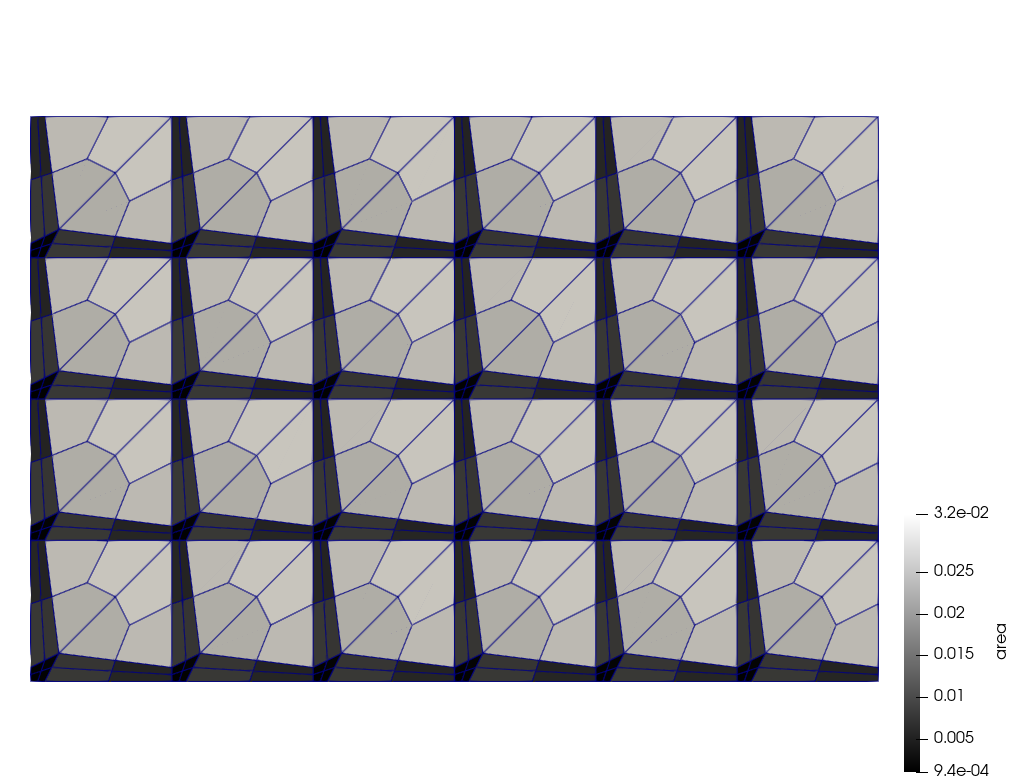
\includegraphics[width=12cm]{python_codes/fieldstone_174/images/area}\\
{\captionfont Example of a $6 \times 4$-cell mesh counting 432 elements and 473 nodes.}
\end{center}


